\documentclass[letterpaper,12pt]{article}
\usepackage{hyperref}

\usepackage{tabularx}

%\usepackage{doublespace}
%\setstretch{1.2}

\usepackage{helvet}
\usepackage{times}
\usepackage{courier}
\usepackage{relsize}
\usepackage{graphicx}
\usepackage{xspace}
\usepackage[T1]{fontenc}
\usepackage{mycv}
\usepackage[top=15mm,left=15mm,right=15mm,bottom=15mm]{geometry}
\begin{document}

\pagestyle{empty}

%Ueberschrift
\begin{center}
{\huge\textsc{Curriculum Vitae}}
\vspace{0.7\baselineskip}

{\Large\textsc{Masataro Asai}}
\vspace{0.5\baselineskip}

% \large
 {
Doctoral Student, Department of General Systems Studies,

Graduate School of Arts and Sciences, University of Tokyo.
}

\vspace{0.4\baselineskip}

 % Male, born March 28th, 1990. Japanese. \\
 % Address: Saginuma-Viola 201 6-23-18 Arima Miyamae-ku Kawasaki Kanagawa, Japan. \\
 % Phone: +81-44-856-9009 \\
 guicho2.71828@gmail.com, +81-50-5534-1357 (Skype: guicho2.71828)\\
 \url{http://guicho271828.github.io/}
\end{center}

\section{Main Research Interest}

\textbf{Domain-independent search/planning/reasoning. Marrying deep learning to classical AI.}

\begin{figure}[h]
 \centering
 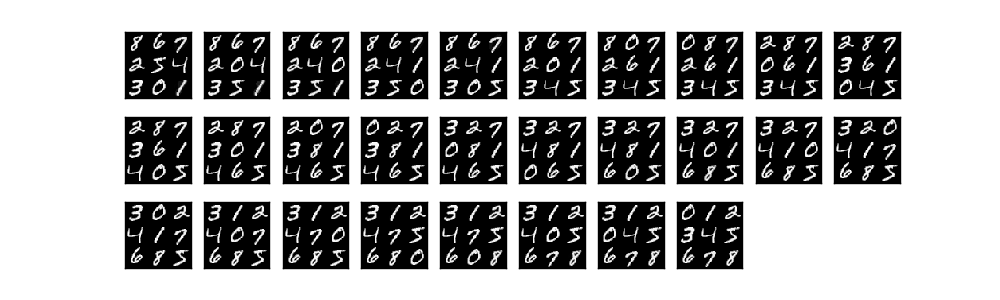
\includegraphics[width=\textwidth]{img/static/blind.png}
 \caption{Result of visually solving 8-puzzle using Deep Neural Network and Classical Planner}
\end{figure}

\section{Education}

\begin{CV}
 \item[04/2013--03/2018] (expected) \textit{Ph.D, M.A.} (received on 03/2015).
 Artificial Intelligence, Heuristic Search, Planning, Scheduling, Optimization.
 {\small % Masters Thesis: \emph{Automated Cyclic Planning for Large Scale Planning Problems}; 
 Advisor: A. Fukunaga}

 \item[04/2009--03/2013] B.Eng in Traffic Simulation.
 Multi-Agent Model, Spatial Search.
 {\small % Thesis: \emph{Distributed Cooperative Agents in Microscopic
 % Traffic Simulation using St-RRT};
 Advisor: S. Yoshimura. H. Fujii.}
\end{CV}

\section{Awards}

\textbf{Research Fellow (DC2), Japan Society for the Promotion of Science} (Equivalent of NSF Grant in Japan; stipends and individual research budget of 10000 USD/year)(Apr. 2016-)


% One of my planning domain CELL-ASSEMBLY is added to SIGAPS ``Real and
% Realistic Planning Domains'' by Patrik Haslum at
% \url{http://users.cecs.anu.edu.au/~patrik/sigaps/index.php?n=Main.RealDomains}
% .

\renewcommand{\refname}{Selected Publications}

{
% \setlength{\bibsep}{-0.1em}
% \setlength{\parsep}{-0.1em}
% \setlength{\baselineskip}{-0.1em}
% \setlength{\itemsep}{-0.1em}
\let\uline\relax
\nocite{Asai2017b}
\nocite{Asai2017}
\nocite{Asai2016b}
\nocite{Asai2016}
\nocite{Asai2015}
\nocite{Asai2014}

% \nocite{Endo2016}
% \nocite{Asai2014b}

\bibliographystyle{unsrt}
\bibliography{asai-references}
}


\section{Work Experience}

\begin{CV}
\item[08/2016--11/2016] Research Internship at IBM Research Ireland.
 Project name: Robust Activity Planning and Scheduling with Multi-Modal Travel.
 Developed an efficient algorithm for multi-worker routing.

\item[03/2014--09/2014] Internship at LogicVein.inc,
 % LogicVein is
 a developer of a Configuration Management System
 for network devices.
 % , an award-winning software that allows the users to
 % efficently manage the complex network configurations of remote routers and switches.
 % Useful batch orders can be triggered by their intuitive graphical interface.
 Worked on % . The materials
 % consist of: advertisement leaflets, blog articles and
 a technical product manual (>200 pages long) %  The materials
 % contain both the Japanese and English documents. Some staff are
 % native English speakers born in United States, who checked and highly
 % evaluated the quality of the English translation.
 % and converted it into 
 % i also converted the Microsoft Word documents into
 % plain-text documents to set up a publishing system.  It compiles the
 % document into a \LaTeX{}-based pdf and multiple
 and its HTML5 conversion.

% \item[04/2013--08/2013] Teaching Assistant in ``Experiments in
%  Information and Environmental Sciences'', under
%  Assoc.\ Prof.\ Haruo Saito.
%  % Students are required to
%  % conduct a specific experiment each week. Experiments include reading
%  % the data from the various sensors and importing it to a computer,
%  % during which the students are required to make use of digital circuits.
%  % Tasks also include measuring the output of comparators, invert
%  % amplifiers and filters that must be built by the students.
%  Students have assembled and calibrated the analog or digital
%  circuits to read the physical values of experimental equipments.

% \item[04/2012--08/2012] Teaching Assistant in ``Field Work -
%  Introductory Course on Automobiles'', under
%  Prof.\ Kohei Kusaka.
%  % The students learn the mechanism and the engineering
%  % design decision of vehicles through vehicle maintenance experience.
%  % prepared the maintainance materials such as lubricant, sealing and
%  % oil filters, moved the vehicle which will be used for maintainance, and
%  Lectured on basic safety measure and the mechanism of vehicles.

\item[12/2011--09/2012] Internship at Metamoji.inc.  Prototyped a
  drawing-chat system for iPad. Both the server/client sides are
  written in Javascript with Node.js and Titanium Mobile.
\end{CV}


\section{Technical Skill}

\begin{CV}
 \item[Programming Paradigm:] %Familiarity with all of: 
 Object-Oriented programming,
 Functional programming,
 Logic / Rule-based programming,
 Metaprogramming, low-level optimization,
 Domain Specific Language(DSL) development, compile-time optimization.
 \item[Development:] Git, GitHub Flow, Test-Driven Development and Continuous Integration (Travis-CI / CircleCI).
 \item[Languages:]
 (Professional) Common Lisp, C++, Bash, Javascript / Coffeescript, C,
 (Intermediate) Java, Python,
 (Elementary)   Ruby
 % \item[Hardware skill:]
 % Digital and Analog circuits, microcontrollers(Arduino,PIC), machining, welding
 \item[Frameworks:] TensorFlow, Cloud services (Amazon AWS, Torque/PBS, OpenLava, cfncluster),
 Node.js% , Titanium Mobile
\end{CV}

\section{Language Ability}

\begin{CV}
 % \item[Japanese:] native
 \item[English:] TOEFL 105/120 (Reading:29/30, Listening:29/30,
 Speaking:22/30, Writing:25/30, Dec 2014).
 % I enjoy daily discussion on Reddit, Github, Skype and IRC channels.
\end{CV}

\section{Community Services / Other activities}

(present) \href{https://github.com/guicho271828}{Open source activities on Github}.

(2016-) AAAI Student Member. Reviewer for ICAPS (2016), AAAI (2015).

(2015) \href{https://github.com/guicho271828/eazy-opencl}{eazy-opencl}
: Common Lisp interface to OpenCL 2.0 (GPGPU language similar to CUDA).

(2015) Contributer of \href{https://github.com/pocl/pocl}{POCL},
a vender-agnostic Portable OpenCL implementation in C and C++.

(2015) \href{https://github.com/guicho271828/trivia}{trivia},
\href{https://github.com/guicho271828/trivia.balland2006}{trivia.balland2006}
: An extensible and fast pattern matching compiler in Common Lisp.

(2012) Macascript : a homoiconic language that compiles into javascript.

(2013--present)
 Compute cluster maintainance and management (80 cores) with NFS/NIS/Torque-PBS.
 Live monitoring/power consumption management.
 Secure VPN network over the campus.

(2011--2012) Mechanical engineering under project professor Kohei Kusaka (former World Rally
 Championship co-driver):
 Full engine modification \& rebuilding of 1.8 liter Mazda BP engine,
 fuel map / ignition timing optimization, map visualization and
 variable resonance intake system (Arduino).

(2011) Certification in ``basic course on machining technique'' by Prof. Ryu Chikayama.

% (2005--2007) Development of Bipedal robot with embedded microcontroller
% (Microchip\textregistered PIC and analog servo motors)


% \section{Undergraduate Thesis Abstract}
% 
% {\small
% In large-scale traffic simulation,
% microscopic multiagent model simulates the behavior of each car (an agent)
% to produce the macroscopic emergent phenomena, e.g.\  traffic-jams,
% % The accuracy of the model are validated through
% % the comparison between the k-q (traffic density to average velocity)
% % curves of simulated and actual environments.
% % which can be heavily affected by the agent behavior.
% and the development of realistic agent model is the key to maintain the simulation accuracy.
% We proposed a coorperative agent model based on Spatiotemporal RRT(St-RRT)
% and evaluated the effectiveness of our approach.
% }
% 
% \section{Masters Thesis Abstract}
% 
% {\small
% In Automated Planning \& Scheduling (P\&S),
% domains such as factory assembly requires the program to
% assemble many identical instances of a particular product.
% While modern classical
% planners can generate assembly plans for single instances of a complex
% product, generating plans to manufacture many instances of a product is
% beyond the capabilities of standard planners. We proposed ACP, a system
% which, given a model of a single instance of a product, automatically
% reformulates and solves the problem as a cyclic planning problem.  We
% showed that our ACP system can successfully generate
% cyclic plans for problems which are too large to be solved directly
% using standard planners.
% }


\end{document}
